
%\documentclass[calculator,allquestions,datasheet,solutions]{exam_newMarcus2}
\documentclass[calculator,allquestions,datasheet,mock,solutions]{exam_newMarcus2}

% The full list of class options are
% calculator : Allows approved calculator use.
% datasheet : Adds a note that data sheet are attached to the exam.
% handbook : Allows the use of the engineering handbook.
% resit : Adds the resit markings to the paper.
% sample : Adds conspicuous SAMPLE markings to the paper
% solutions : Uses the contents of \solution commands (and \solmarks) to generate a solution file
% mock: For a mock-exam paper

\usepackage{pdfpages}  
\usepackage{lscape,comment} 
 
\coursecode{EX3029}%%
\coursetitle{Chemical Thermodynamics}
 
\examtime{14.00--16.00}%
\examdate{27}{10}{2016}% 
\examformat{Candidates must attempt \textit{all} questions, each of which carries equal (20) marks.  All thermodynamic symbols have their usual meanings unless otherwise stated.}

\newcommand{\frc}{\displaystyle\frac}
\newcommand{\br}[1]{\!\left( #1 \right)}
\newcommand{\abs}[1]{\left| #1 \right|}
\newcommand{\fracd}[2]{\frac{\mathrm{d} #1}{\mathrm{d} #2}}
\newcommand{\fracp}[2]{\frac{\partial #1}{\partial #2}}
\renewcommand{\d}[1]{\mathrm{d} #1 } 
\newcommand{\Ma}{\mathrm{M\!a}} 
\newcommand{\Partial}[3][error]{\left(\frc{\partial #1}{\partial #2}\right)_{#3}}
\newcommand{\mfr}[3][error]{#1_{#2}^{\left(#3\right)}} 



\begin{document}


%%%
%%% Question 03
%%%
\begin{question}
In a petrochemical plant, propane is transferred from the storage tank to a dehydrogenation reactor. 
\begin{enumerate}[(a)]
%
   \item Determine the volumetric flow rate $\left(\text{in m}^{3}.\text{h}^{-1}\right)$ of propane at 423 K and 71 bar using the Soave-Redlich-Kwong equation of state (SRK-EOS),
       \begin{displaymath}
           P = \frc{R T}{V - b} - \frc{\alpha a}{V\left(V+b\right)},
       \end{displaymath} 
       with
       \begin{eqnarray}
          &&a = 0.42747\frc{\left(R T_{c}\right)^{2}}{P_{c}},\;\; b = 0.08664\frc{R T_{c}}{P_{c}},\;\; \alpha = \left[ 1 + m\left(1-\sqrt{T_{r}}\right)\right]^{2}\;\;\text{ and } \nonumber \\
           && m = 0.48508 + 1.55171\omega - 0.1561\omega^{2}. \nonumber
       \end{eqnarray}
       where $R\left(=8.314\times 10^{-5}\frc{\text{bar.m}^{3}}{\text{mol.K}}\right)$ is the molar gas constant and $V$ is the molar volume. The transfer is conducted at a molar flow rate of 10$^{5}$ mol.h$^{\text{-1}}$. Use the ideal gas law for the initial estimate of the molar volume of propane. Data for propane: $T_{c}=$ 369.9 K, $P_{c}=$ 42.61 bar and $\omega=$ 0.152.~\marks{13}
%======================
         \solution{The first step to solve the problem is to calculate the parameters for the SRK-EOS:\solmarks{8/13}
     \begin{eqnarray}
        a &=& \frc{\left(R T_{c}\right)^{2}}{P_{c}} = 0.42748\frc{\left[8.314\times 10^{-5}\frc{\text{bar.m}^{3}}{\text{mol.K}} \times 369.9\text{ K}\right]^{2}} {42.61\text{ bar}} = 9.4884\times 10^{-6} \frc{\text{m}^{6}\text{bar}}{\text{mol}^{2}}\nonumber \\
        b &=& 0.08664\frc{R T_{c}}{P_{c}} = 6.2532\times 10^{-5} \frc{\text{m}^{3}}{\text{mol}} \nonumber \\
        m &=& 0.48508 + 1.55171\omega - 0.1561\omega^{2} = 0.7173 \nonumber \\
        \alpha &=& \left[ 1 + m\left(1-\sqrt{T_{r}}\right)\right]^{2} = 0.9029 \;\text{ with } T_{r}=\frc{T}{T_{c}} = 1.1436 \nonumber 
     \end{eqnarray}
     Substituting these parameters in the SRK-EOS,
       \begin{displaymath}
           P = \frc{R T}{V - b} - \frc{\alpha a}{V\left(V+b\right)},
       \end{displaymath} 
       leads to $V=2.8876\times 10^{-4}\frc{\text{m}^{3}}{\text{mol}}$.~\solmarks{2/13} The volumetric flow rate is~\solmarks{3/13}
       \begin{displaymath}
           \dot{v} = 2.8876\times 10^{-4}\frc{\text{m}^{3}}{\text{mol}} \times 10^{5} \frc{\text{mol}}{\text{h}} = 28.88 \frc{\text{m}^{3}}{\text{h}}
       \end{displaymath} 
}
%
    \item One mole of propane gas is expanded from 10$^{-3}$ to 4.0$\times$10$^{-2}$ m$^{3}$ in a heating bath at 100$^{\circ}$C. The expansion is not reversible and the heat extracted from the bath is 0.6 kJ. Determine the work for the expansion using the van der Waals equation of state (vdW-EOS),
       \begin{displaymath}
           P = \frc{R T}{V - b} - \frc{a}{V^{2}},\text{ with }\; a = \frc{27}{64}\frc{\left(R T_{c}\right)^{2}}{P_{c}}\;\text{ and }\; b=\frc{R T_{c}}{8 P_{c}}.
       \end{displaymath} 
       For your calculation, consider $a=$9.126$\times$10$^{-3}$ m$^{3}$.bar.mol$^{-1}$ and the molar internal energy~\marks{7}
          \begin{displaymath}
             dU = \left[T\left(\frc{\partial P}{\partial T}\right)_{V}-P\right]\d V
          \end{displaymath}
      \solution{ From the First law -- $\Delta U = Q + W$, with the amount of heat transferred given as 600 J/mol. Therefore, we need to evaluate $\Delta U$ to calculate the work. The variation of molar internal energy, 
          \begin{displaymath}
             dU = \left[T\left(\frc{\partial P}{\partial T}\right)_{V}-P\right]\d V
          \end{displaymath}
       In order to obtain $\left(\frc{\partial P}{\partial T}\right)_{V}$, we can differentiate the vdW-EOS with respect to the temperature,\solmarks{2/7}
       \begin{displaymath}
          \left(\frc{\partial P}{\partial T}\right)_{V} = \frc{R}{V-b}
       \end{displaymath}
       and the term in the brackets is,\solmarks{1/7}
       \begin{displaymath}
          T\left(\frc{\partial P}{\partial T}\right)_{V}-P = \frc{a}{V^{2}}
       \end{displaymath}
       Therefore, the variation of molar internal energy is~\solmarks{2/7}
       \begin{eqnarray}
         \Delta U &=& \int\limits_{0.001\text{ m}^{3}}^{0.04\text{ m}^{3}}\left[T\left(\frc{\partial P}{\partial T}\right)_{V}-P\right]\d V = \int\limits_{0.001\text{ m}^{3}}^{0.04\text{ m}^{3}} \frc{a}{V^{2}} \d V = -\left.\frc{a}{V}\right|_{0.001\text{ m}^{3}}^{0.04\text{ m}^{3}} \nonumber \\
                  &=& 9.126\times 10^{-3}\frc{\text{m}^{3}.\text{bar}}{\text{mol}} = 912.60\text{ J.mol}^{-1}, \nonumber
       \end{eqnarray}
       And the work is $W= \Delta U - Q=312.60\text{ J.mol}^{-1}$~\solmarks{2/7}

}
%
\end{enumerate} 
%
\end{question}

\clearpage




%%%
%%% Question 01 (Mock)
%%%
\begin{question}
%
\begin{enumerate}[(a)] % (Shapiro 2.34) 
\item A closed system with 0.09 kg of air undergoes a polytropic process from $P_{1}$ = 138 kPa, $v_{1}$=0.72 m$^{3}$.kg$^{-1}$ to a final state where $P_{2}$ = 552 kPa, $v_{2}$ = 0.25 m$^{3}$.kg$^{-1}$.  Determine the work (in $kJ$) required for this compression.~\marks{8} 
\solution{
First stage is to calculate the polytropic coefficient,
\begin{displaymath}
P_{1}v_{1}^{n} = P_{2}v_{2}^{n} \Longrightarrow {\bf n} = \frc{\ln P_{2}/P_{1}}{\ln v_{1}/v_{2}} {\bf = 1.31}
\end{displaymath}~\solmarks{4/8}
Now, calculating the work with $V_{i}=v_{i}\times m$, thus V$_{1}=0.0648$ m$^{3}$ and V$_{2}=0.0225$ m$^{3}$:
\begin{eqnarray}
{\bf W }&=& -\int\limits_{V_{1}}^{V_{2}} P dV = -\int\limits_{V_{1}}^{V_{2}} \frc{C}{V^{n}} dV = -\left.C \frc{V^{1-n}}{1-n}\right|_{V_{1}}^{V_{2}} = -\frc{P_{2}V_{2}^{n}V_{2}^{1-n}-P_{1}V_{1}^{n}V_{1}^{1-n}}{1-n} = -\frc{P_{2}V_{2}-P_{1}V_{1}}{1-n} \nonumber \\
   &=& {\bf 11.214 kJ} \nonumber
\end{eqnarray} ~\solmarks{4/8}}



\item Calculate the compressibility factor ($Z$) of chloroform vapour at 450 K and 20 bar (molar volume of 1.35$\times$10$\left.^{-3}\text{ m}^{3}.\text{mol}^{-1}\right)$ using the Soave-Redlich-Kwong equation of state. If you are using an iterative method (i.e., hand-calculation), do use the ideal gas equation of state to estimate the initial guess, $Z_{0}$, and stop at the second iteration, $Z_{2}$. Properties of chloroform are: T$_{c}$ = 537 K, P$_{c}$ = 5328.68 kPa and $\omega$ =0.218 (accentric factor).~\marks{12}
\solution{ The generic form of $Z$ is,
\begin{displaymath}
Z = 1+ \beta - q\beta\frc{Z - \beta}{\left(Z+\epsilon\beta\right)\left(Z+\sigma\beta\right)}\;\;\text{ with} \;\; \beta = \Omega \frc{P_{r}}{T_{r}}\;\;\text{ and}\;\; q=\frc{\Psi\alpha}{\Omega T_{r}}
\end{displaymath}
For SRK with {\bf T$_{r}$=0.8380}, {\bf P$_{r}$=0.3754}, {\bf $\beta$=3.88$\times$10$^{-2}$} and {\bf $q$=6.7274}~\solmarks{2/12},
\begin{displaymath}
{\bf Z = 1 + \beta - q\beta\frc{Z-\beta}{Z^{2}+\beta Z}}
\end{displaymath}~\solmarks{2/12}
The equation is non-linear and to find the root we can apply Newton-Raphson method 
\begin{displaymath}
Z_{i} = Z_{i-1} - \frc{\mathcal{F}\left(Z_{i-1}\right)}{d\mathcal{F}/dZ \left(Z_{i-1}\right)}
\end{displaymath}
with,
\begin{eqnarray}
&& \mathcal{F}\left(Z\right) = Z - \left[ 1 + \beta - q\beta\frc{Z-\beta}{Z^{2}+\beta Z}\right] \nonumber \\
&& \frc{d\mathcal{F}}{dZ}\left(Z\right) = 1 + q\beta \frc{\beta^{2}+2\beta Z- Z^{2}}{\left(Z^{2}+\beta Z\right)^{2}} \nonumber
%\frc{q\beta\left(Z^{2}\beta +Z\right)-q\beta Z\left(2Z + \beta\right)}{\left(Z^{2}+\beta Z\right)^{2}} + \frc{q\beta^{2}\left(2Z+\beta\right)}{\left(Z^{2}+\beta Z\right)^{2}} \nonumber
\end{eqnarray} 
%as initial guess, we can use the generic real gas EOS, $PV=Z_{0}RT \Longrightarrow$ $Z_{0}=0.7217$. Thus 
\begin{center}
{\bf $Z_{1}$ = 0.7184}~\solmarks{4/12} \\
{\bf $Z_{2}$ = 0.7160}~\solmarks{4/12} \\
$\cdots \cdots \cdots $ \\
\textcolor{red} {or (using calculator) }{\bf $Z_{22}$ = 0.7088}~\solmarks{\textcolor{red}{8/12}} \\

\end{center}
} 

\end{enumerate}

\end{question} 
\clearpage


%%%
%%% Question 01 (Fluid Phase Equilibrium)
%%% LectureNotes_Nguyen (pg 89)
%%%
\begin{question}
Given the van der Waals equation of state (vdW EOS),
     \begin{displaymath}
         P = \frc{RT}{V-b} - \frc{a}{V^{2}},
     \end{displaymath} 
     \begin{enumerate}[(a)]
         \item Show that the vdW EOS can be expressed as a cubic polynomial equation in $Z$ (compressibility coefficient),
             \begin{displaymath}
                  Z^{3} -(1+B)Z^{2} +AZ -AB = 0,
             \end{displaymath}
             with $B=bP/(RT)$, $A=aP/(RT)^{2}$ and $R\left(=8.314\times 10^{-5}\frc{\text{bar.m}^{3}}{\text{mol.K}}\right)$ is the molar gas constant~\marks{7}
%==========================
\solution{We can rearrange the vdW EOS,~\solmarks{2/7}
\begin{displaymath}
   P = \frc{RT}{V-b} - \frc{a}{V^{2}} \Longrightarrow \frc{PV}{RT} = \frc{V}{V-b} - \frc{a}{RTV} = \frc{1}{1-\frc{b}{V}} - \frc{a}{RTV}
\end{displaymath}
Eliminating $V$ as $V=ZRT/P$,~\solmarks{1/7}
\begin{displaymath}
   Z = \left(1-\frc{bP}{ZRT}\right)^{-1} - \frc{aP}{Z\left(RT\right)^{2}} = \frc{ZRT}{ZRT-bP}-\frc{aP}{Z\left(RT\right)^{2}}
\end{displaymath}
Manipulating this expression,~\solmarks{3/7}
\begin{eqnarray}
   && Z^{2}R^{2}T^{2}\left(ZRT-bP\right) = Z^{2}\left(RT\right)^{3} - aP\left(ZRT-bP\right) \nonumber \\
   && Z^{3} - \frc{bP}{RT}Z^{2} - Z^{2} -\frc{aP}{\left(RT\right)^{2}}Z + ab\frc{P^{2}}{\left(RT\right)^{3}} = 0 \nonumber
\end{eqnarray}
with $B=bP/(RT)$, $A=aP/(RT)^{2}$,~\solmarks{1/7}
\begin{displaymath}
Z^{3} -(1+B)Z^{2} +AZ -AB = 0 
\end{displaymath}
}
%==========================

\item Calculate the fugacity of gaseous CO$_{2}$ at 310 K and 1.4 MPa using the vdW EOS, with $a=$ 0.3658 Pa.m$^{6}$.mol$^{-2}$, $b=$ 4.286$\times$10$^{-5}$ m$^{3}$.mol$^{-1}$. Given,
\begin{displaymath}
\ln{\left(\frc{f}{P}\right)} = -\ln{\left(1-\frc{b}{V}\right)} - \frc{a}{RTV} - \ln{Z} +\left(Z-1\right).
\end{displaymath}
Use the largest real root of the cubic polynomial equation in $Z$ to represent the gaseous phase.~\marks{13}

%====================
\solution{Solving the cubic polynomial in $Z$, with $B=bP/(RT)$ and $A=aP/(RT)^{2}$,~\solmarks{5/13}
\begin{eqnarray}
Z^{3} -(1+B)Z^{2} +AZ -AB = 0 & \Longrightarrow& A = 7.7095\times 10^{-2}\; ;\; B = 2.3281\times 10^{-2} \nonumber \\ 
 &\Longrightarrow& Z = 0.9436 \nonumber
\end{eqnarray}
Now for the fugacity equation, either
\begin{eqnarray}
&& \ln{\left(\frc{f}{P}\right)} = -\ln{\left(1-\frc{b}{V}\right)} - \frc{a}{RTV} - \ln{Z} +\left(Z-1\right) \nonumber \\
&& \text{or} \nonumber \\
&&  \ln{\left(\frc{f}{P}\right)} = -\ln{\left(1-\frc{B}{Z}\right)} - \frc{A}{Z} - \ln{Z} +\left(Z-1\right) \nonumber
\end{eqnarray}
leads to $f =\; 1.32\times 10^{6}$ Pa.~\solmarks{8/13}

}
%====================
%
\end{enumerate}
%
\end{question}

\clearpage


%%%
%%% Question 02
%%%
\begin{question}
In a saturated liquid mixture of benzene and toluene containing 45 mol$\%$ of benzene, determine:
\begin{enumerate}[(a)]
%
   \item Temperature and composition of the first bubble at 200 kPa.~\marks{5}
%======================
         \solution{ The molar constraint of vapour composition is
\begin{displaymath}
   \sum\limits_{i=1}^{2}y_{i} = y_{1} + y_{2} = 1,
\end{displaymath}
and replacing the Raoult law, $y_{i}=\frac{x_{i}P_{i}^{\text{sat}}}{P}$, in the constraint relation,
\begin{eqnarray}
   P &=& x_{1}P_{1}^{\text{sat}} + x_{2}P_{2}^{\text{sat}} \nonumber \\
     &=& x_{1}\exp{\left(A_{1}-\frc{B_{1}}{T+C_{1}}\right)} + x_{2}\exp{\left(A_{2}-\frc{B_{2}}{T+C_{2}}\right)} \nonumber
\end{eqnarray}
Solving this non-linear equation we obtain the bubble temperature of the benzene-toluene mixture as $T=391.79$ K.~\solmarks{3/5} In order to calculate the compositions, we should use the Raoult's relation,~\solmarks{2/5}
\begin{displaymath}
     y_{1} = \frc{x_{1}P_{1}^{\text{sat}}}{P} = 0.6503 \Longrightarrow y_{2} = 0.3497
\end{displaymath}
}
%
   \item Pressure and composition of the first bubble at 400 K.~\marks{5}
%======================
         \solution{ The molar constraint of vapour composition is
\begin{displaymath}
   \sum\limits_{i=1}^{2}y_{i} = y_{1} + y_{2} = 1,
\end{displaymath}
and replacing the Raoult law, $y_{i}=\frac{x_{i}P_{i}^{\text{sat}}}{P}$, in the constraint relation,
\begin{eqnarray}
   P &=& x_{1}P_{1}^{\text{sat}} + x_{2}P_{2}^{\text{sat}} \nonumber \\
     &=& x_{1}\exp{\left(A_{1}-\frc{B_{1}}{T+C_{1}}\right)} + x_{2}\exp{\left(A_{2}-\frc{B_{2}}{T+C_{2}}\right)} \nonumber
\end{eqnarray}
Solving this equation for $T = 400$ K results in $P=245.28$ kPa.~\solmarks{3/5} In order to calculate the compositions, we should use the Raoult's relation,~\solmarks{2/5}
\begin{displaymath}
     y_{1} = \frc{x_{1}P_{1}^{\text{sat}}}{P} = 0.6461 \Longrightarrow y_{2} = 0.3539
\end{displaymath}
         }
         %
  \item Sketch the $P-xy$ diagram of this mixture at 400 K, indicating (with values) bubble and dew point pressures, liquid and vapour compositions and saturated pressures of both components.~\marks{10}
    \solution{ Bubble point pressure and compositions of the vapour vapour phase were obtained in (b). Dew point pressure at 400K can be obtained from
      \begin{displaymath}
        \sum\limits_{i=1}^{2} x_{i} = 1 = \frc{y_{1}P}{P_{1}^{\text{sat}}} + \frc{y_{2}P}{P_{2}^{\text{sat}}},
      \end{displaymath}
      leading to $\mathbf{P=209.98\text{ kPa}}$~\solmarks{3/10} with composition of the liquid phase of $\mathbf{x_{1}=0.2683}$ and $\mathbf{x_{2}=0.7317}$~\solmarks{2/10}.$P-xy$ diagram at constant temperature of 400 K with bubble and dew point pressures, liquid and vapour compositions and saturated pressures of both components are,~\solmarks{5/10}
       \begin{center}
         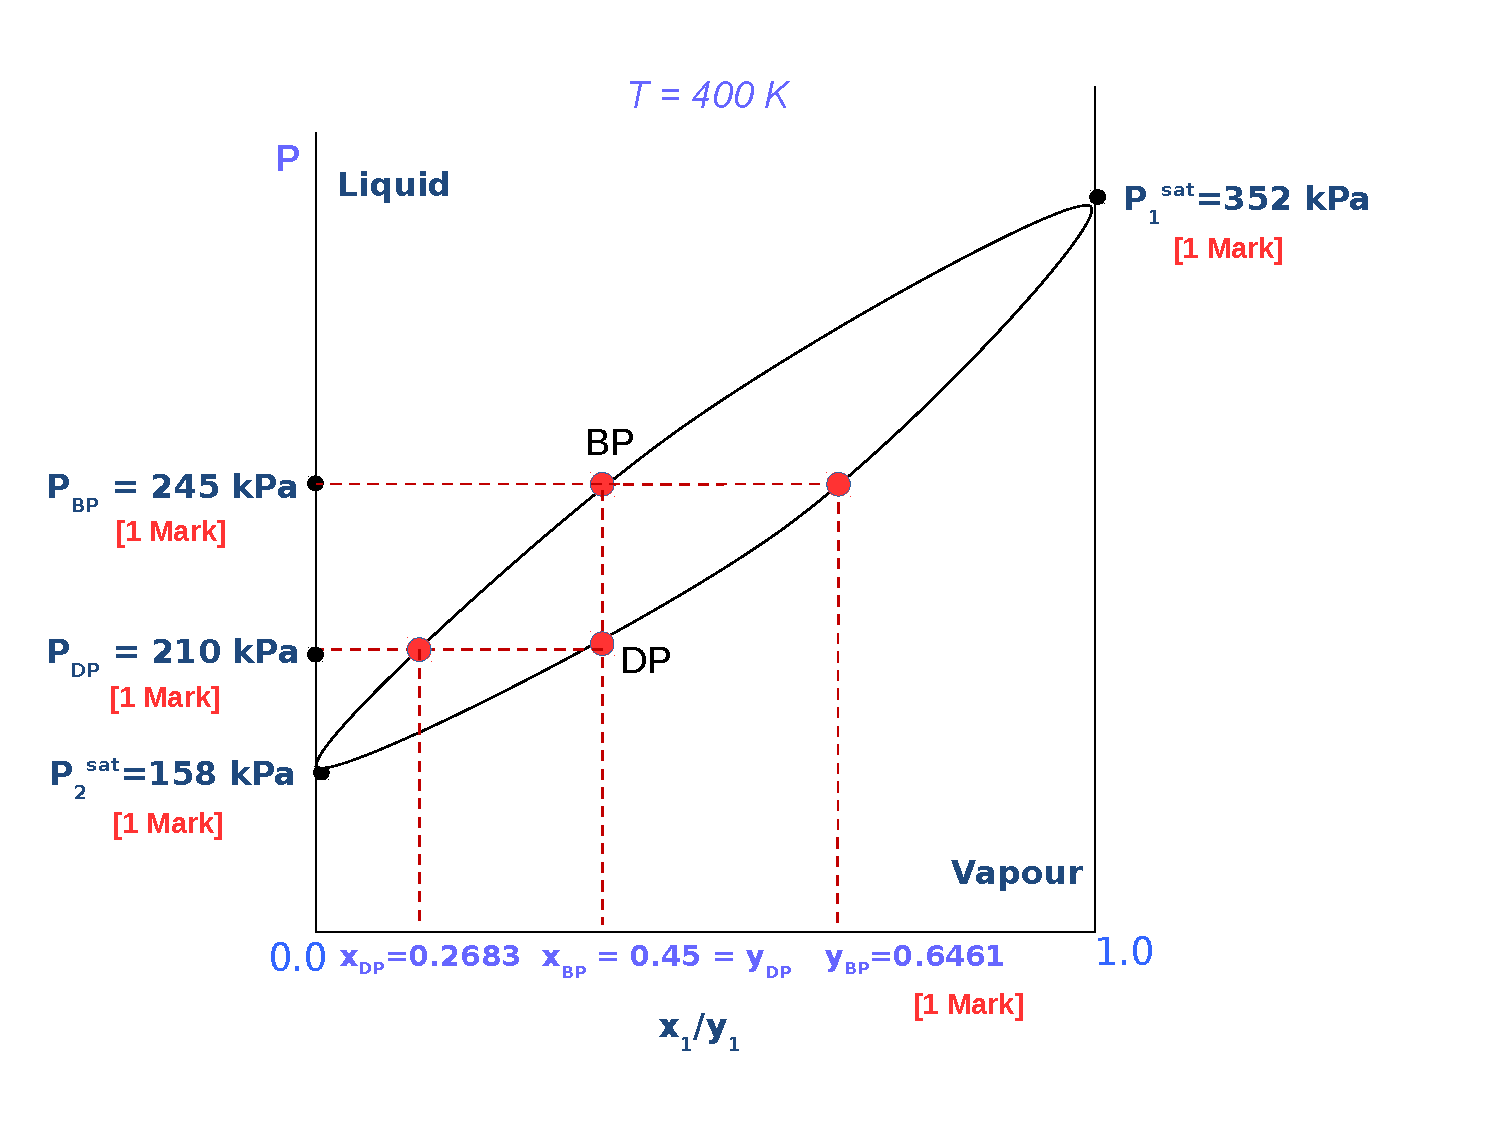
\includegraphics[width=\columnwidth, clip]{./Pics/VLE_Pxy_Diagram}
       \end{center}}

%
\end{enumerate}

For this problem, benzene and toluene mixtures may be considered as ideal and you should use,
\begin{displaymath}
   \ln P_{i}^{\text{sat}} = A_{i} - \frc{B_{i}}{T + C}
\end{displaymath} 
with [P] = bar, [T] = K, [B] = K and [C] = K.
    \begin{center}
       \begin{tabular}{l | c c c}   
           {\bf Species}  &   {\bf A } &  {\bf B } &  {\bf C } \\
           \hline
             Benzene (1)  &  14.1603   &  2948.78  & -44.5633  \\
             Toluene (2)  &  14.2515   &  3242.38  & -47.1806   
       \end{tabular}
    \end{center}
%
\end{question}

\clearpage



\clearpage


%%%
%%% Question 05 (Example 5.2 of NPTEL)
%%%
\begin{question}

\begin{enumerate}[(a)]
   \item Derive an expression for enthalpy change of a gas during an isothermal process assuming that the gas behaves accordingly with the following EOS:
                     \begin{displaymath}
                        Z = 1 + A \frc{P_{r}}{T_{r}},
                     \end{displaymath}
         where $Z$, $A$, $P_{r}$ and $T_{r}$ are constant compressibility factor, arbitrary constant, reduced pressure and temperature, respectively. Also, given the residual enthalpy expression,
                     \begin{displaymath}
                        \frc{H^{R}}{RT_{c}} = - T_{r}^{2}\int\limits_{0}^{P_{r}}\Partial[Z]{T_{r}}{P_{r}}\frc{d P_{r}}{P_{r}},
                     \end{displaymath}
         where $T_{c}$ is the critical temperature.~\marks{8}
         \solution{For this problem we want to derive an expression for enthalpy change of an arbitrary real gas, $\Delta H$, given an EOS. Any thermodynamic property of real gases, $M$, can be expressed as functions of the equivalent ideal gas, $M^{\text{ig}}$, that can be readily obtained, and from residual properties of the gas, $M^{R}$, i.e.,~\solmarks{2/8}
            \begin{displaymath}
                M^{R} = M - M^{\text{ig}}.
            \end{displaymath}
            And for enthalpy changes~\solmarks{1/8}
            \begin{displaymath}
                \Delta H = \Delta H^{\text{ig}} + \Delta H^{R}.
            \end{displaymath}
            Thus we need to find an expression for $\Delta H^{R}$ based on the given equation,~\solmarks{3/8}
                     \begin{eqnarray}
                        \frc{H^{R}}{RT_{c}} &=& - T_{r}^{2}\int\limits_{0}^{P_{r}}\Partial[Z]{T_{r}}{P_{r}}\frc{d P_{r}}{P_{r}} = - T_{r}^{2}\int\limits_{0}^{P_{r}}\Partial[\left(1 + A \frc{P_{r}}{T_{r}}\right)]{T_{r}}{P_{r}}\frc{d P_{r}}{P_{r}} \nonumber \\
                                          &=& - T_{r}^{2}\int\limits_{0}^{P_{r}}\left(-\frc{AP_{r}}{T_{r}^{2}}\right)\frc{d P_{r}}{P_{r}} = AP_{r} \nonumber
                     \end{eqnarray}
           Now, ~\solmarks{2/8}
            \begin{eqnarray}
                \Delta H &=& \Delta H^{\text{ig}} + \Delta H^{R} = \Delta H^{\text{ig}} - \left(H_{2}^{R}-H_{1}^{R}\right) \nonumber \\
                         &=& \Delta H^{\text{ig}} + A\left(P_{r2}-P_{r1}\right)RT_{c} \nonumber
            \end{eqnarray}
         }

   \item In a nuclear power plant, 10 kg.s$^{-1}$ of steam at 30 bar and 400$^{\circ}$C is isentropically expanded in a turbine to 1 bar. Determine:
          \begin{enumerate}
              \item Saturated temperature of the water-steam at 30 bar and 1 bar;~\marks{2}
                  \solution{From the saturated water-steam table, the saturated temperature of water-steam at 30 bar and 1 bar are 233.9$^{\circ}$C~\solmarks{1/2} and 99.63$^{\circ}$C, respectively~\solmarks{1/2}.

                  }
              \item Quality of the water-steam after the expansion;~\marks{5}
                  \solution{ At 30 bar, saturated temperature of water-steam is 233.9$^{\circ}$C $<<<$ 400$^{\circ}$C, therefore the fluid is at superheated state with~\solmarks{2/5}
                     \begin{displaymath}
                       h_{1} = 3230.9 \text{ kJ.kg}^{-1}\;\;\text{ and }\;\; s_{1} = 6.9212\text{ kJ.}\left(\text{kg.}^{\circ}\text{C}\right)^{-1}.
                     \end{displaymath}
                     At 1 bar (from saturated tables), 
                     \begin{eqnarray}
                       h_{f} = 417.46 \text{ kJ.kg}^{-1}\;\;\text{ and }\;\; s_{f} = 1.3026\text{ kJ.}\left(\text{kg.}^{\circ}\text{C}\right)^{-1}, \nonumber \\
                       h_{g} = 2675.5 \text{ kJ.kg}^{-1}\;\;\text{ and }\;\; s_{g} = 7.3594\text{ kJ.}\left(\text{kg.}^{\circ}\text{C}\right)^{-1}. \nonumber
                     \end{eqnarray}
                     The water-steam is isentropically expanded in the turbine, i.e., $s_{2}=s_{1}$, therefore as $s_{f} < s_{2} < s_{g}$, we can conclude that the fluid leaving the turbine is partially condensed. The quality of the vapour can be calculated from~\solmarks{3/5}
                       \begin{displaymath}
                          \mfr[x]{}{V} = \frc{M-\mfr[M]{}{L}}{\mfr[M]{}{V} - \mfr[M]{}{L}} = \frc{s_{2}-s_{f}}{s_{g}-s_{f}} = \frc{6.9212-1.3026}{7.3594-1.3026} = 0.9277
                       \end{displaymath}
                  }
              \item Power generated in the turbine (in MW);~\marks{5}
                  \solution{ Using the quality calculated in (b), we can obtain $h_{2}$,~\solmarks{2/5}
                       \begin{displaymath}
                          \mfr[x]{}{V} = \frc{M-\mfr[M]{}{L}}{\mfr[M]{}{V} - \mfr[M]{}{L}} = \frc{h_{2}-h_{f}}{h_{g}-h_{f}} = \frc{h_{2}-417.46}{2675.5-417.46} = 0.9277\;\;\Rightarrow\;\; h_{2} = 2512.2437\text{ kJ.kg}^{-1}.
                       \end{displaymath}
                       The power produced by the turbine can be obtained from energy balance, i.e.,
                        \begin{displaymath}
                            \text{Output Energy} - \text{Input Energy} = 0 \;\;\Rightarrow\;\; \left(\dot{m}_{w}h_{2}+\dot{W}_{T}\right) - \dot{m}_{w}h_{1} = 0\;\;\Leftrightarrow\;\; \dot{W}_{T} = \dot{m}_{w}\left(h_{1}-h_{2}\right)
                        \end{displaymath}
                        leading to~\solmarks{3/5}
                        \begin{displaymath}
                           \dot{W}_{T} = 7.19\text{ MW}
                        \end{displaymath}
                  }
          \end{enumerate}
                         
\end{enumerate}

\end{question}


\vfill
\paperend



\vfill 



%\begin{comment}
{
  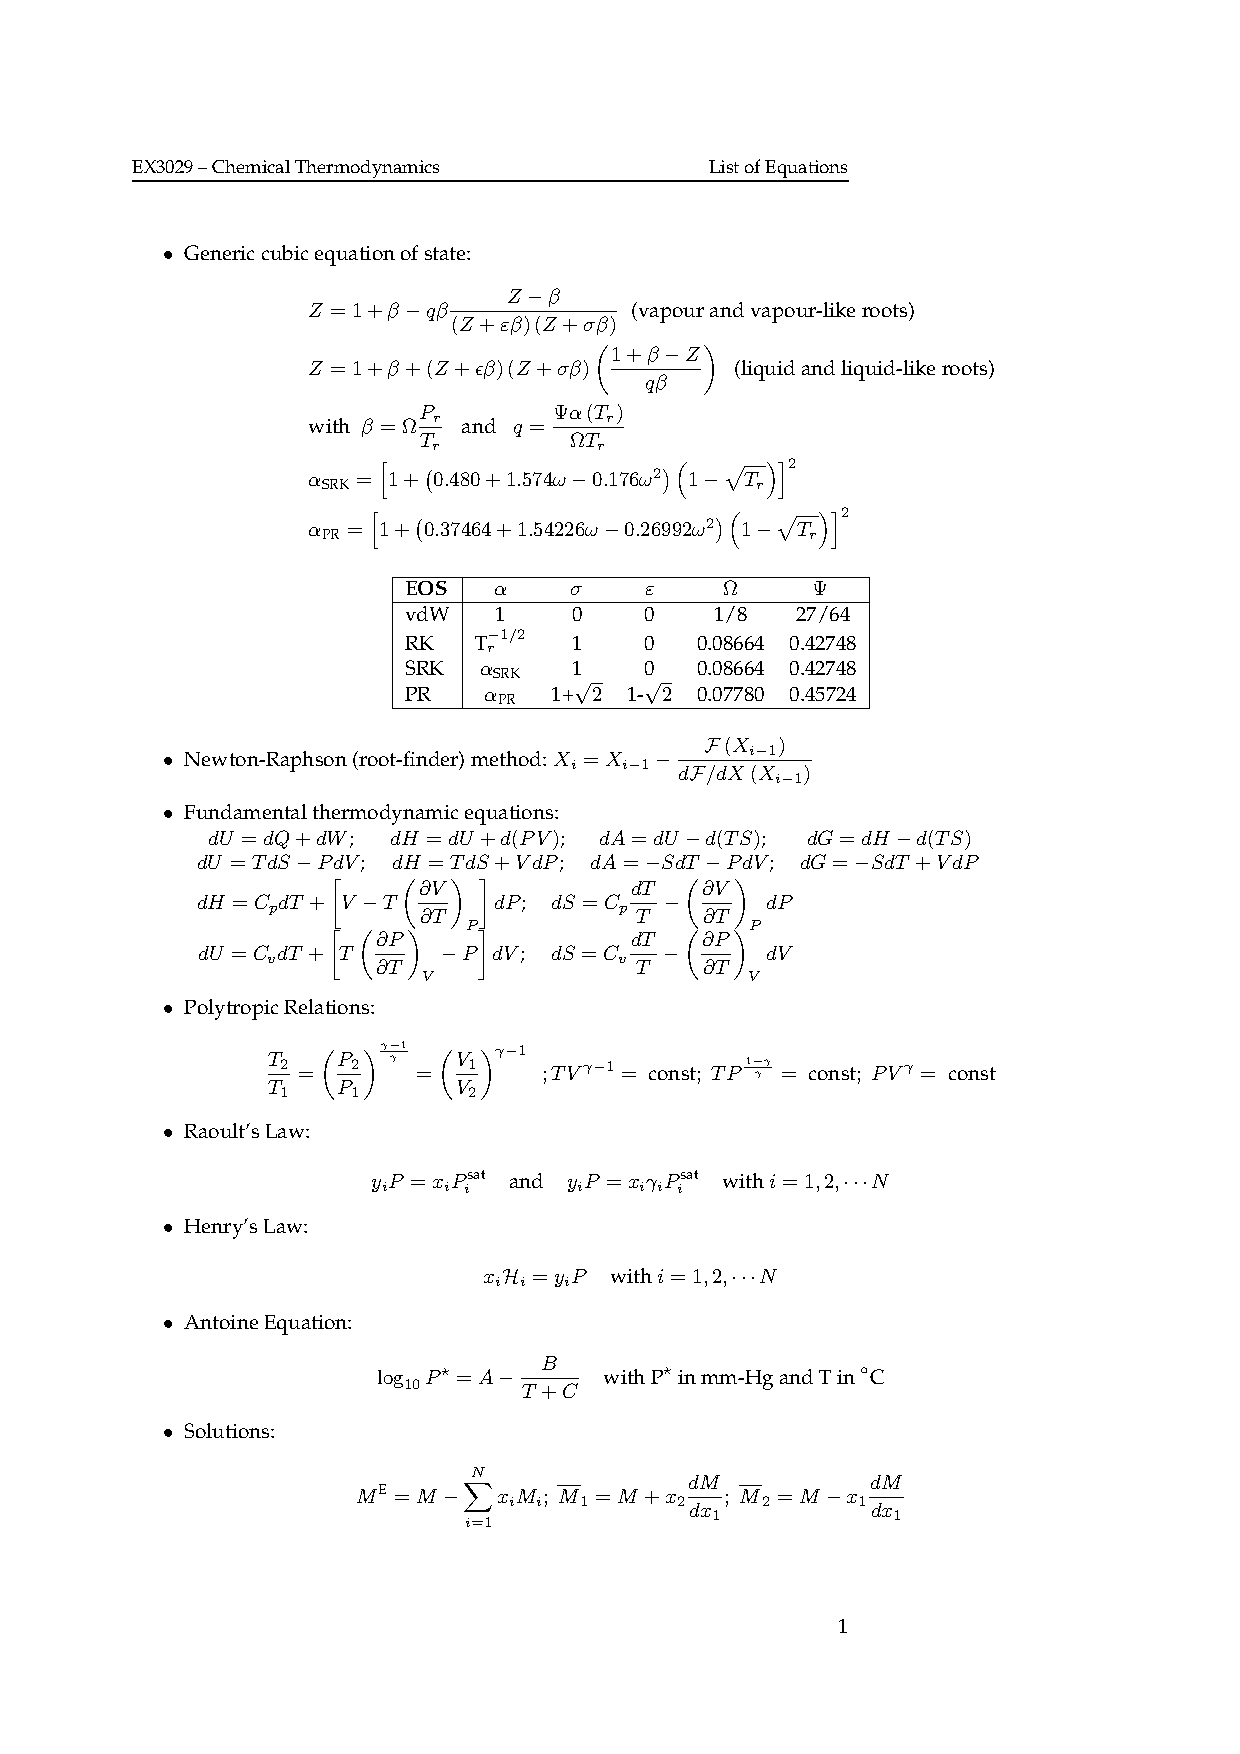
\includepdf[pages=-,fitpaper]{./Pics/EquationsList}
  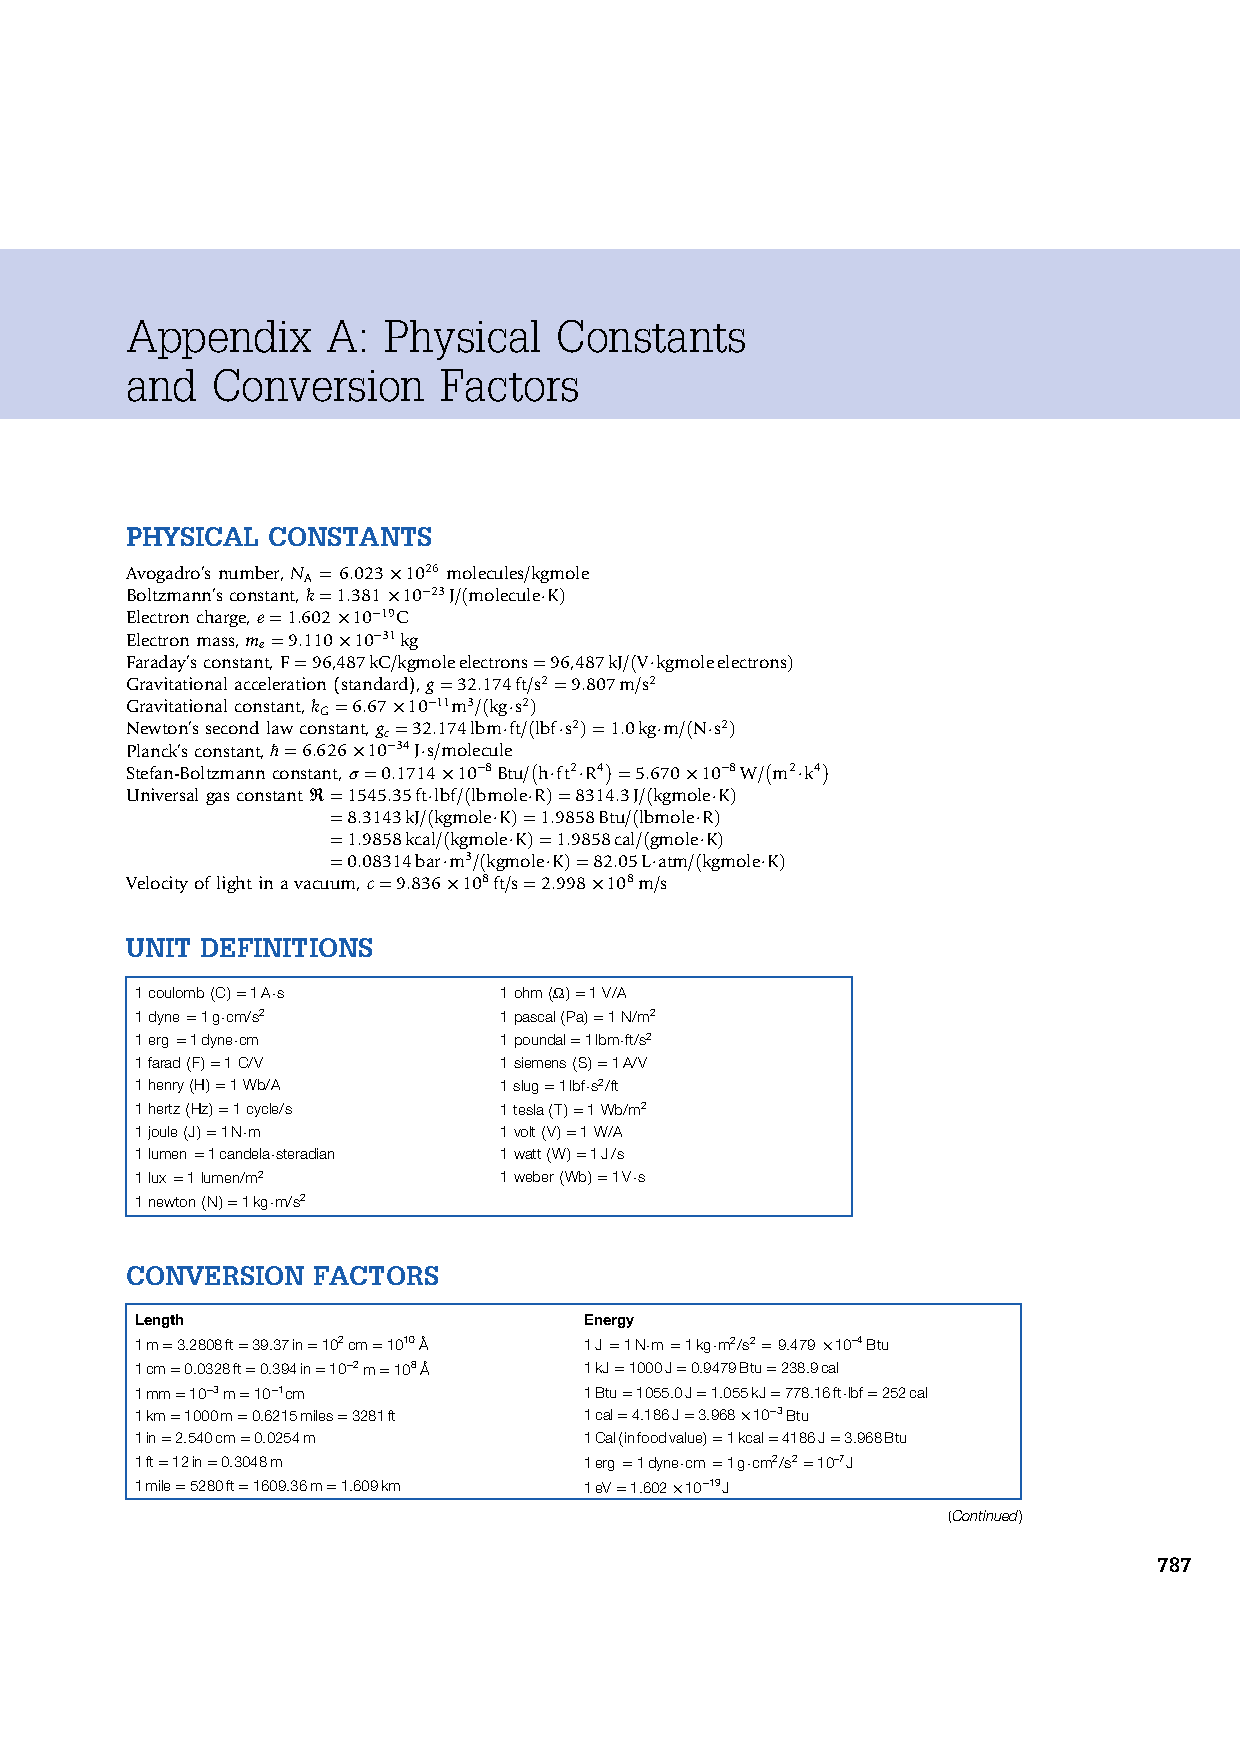
\includepdf[pages=-,fitpaper]{./Pics/SelectedWaterSteam__UnitConv}
}
%\end{comment}



\end{document}
